\section{LTI-Systeme (S.35)}
\begin{list}{$\bullet$}{\setlength{\itemsep}{0cm} \setlength{\parsep}{0cm} \setlength{\topsep}{0cm}} 
	\item Lineare Systeme sind durch die Antworten auf die
	Basissignale bestimmt.
	\item Basissignale müssen linear unabhängig voneinander sein
	\item Alle Eingangs-Funktionen müssen durch eine Linearkombination der
	Basissignale darstellbar sein.\\ $\Rightarrow$ \textbf{Periode des Eingangssignals =	Anzahl Basissignale}
\end{list}

\begingroup
\small
\renewcommand{\arraystretch}{1.3}
\providecommand{\ltikey}[1]{\fcolorbox{red!70!black}{white}{$#1$}}

\noindent
\begin{tabularx}{\linewidth}{|>{\bfseries}l|>{\raggedright\arraybackslash}X|>{\raggedright\arraybackslash}X|}
\hline
Begriff & \textbf{Beschreibung} & \textbf{Zusätzliche Bemerkungen} \\
\hline
System &
Eindeutige Zuordnung von Ausgang (Wirkung) und Eingang (Ursache)
\par
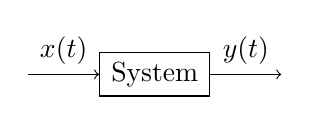
\begin{tikzpicture}[baseline=(b.base)]
  \node[draw,minimum width=1.4cm,minimum height=0.55cm] (b) {System};
  \draw[->] ([xshift=-0.9cm]b.west) -- node[above]{$x(t)$} (b.west);
  \draw[->] (b.east) -- node[above]{$y(t)$} ([xshift=0.9cm]b.east);
\end{tikzpicture}\smallskip
&
Übertragungswege, Filter, Verstärker, Modulatoren, Abtaster
\par
SISO-, MIMO-, SIMO-, MISO-Systeme \\
\hline
Linear &
Linearkombination am Eingang ruft entsprechende Linearkombination am Ausgang hervor
\par\smallskip
\emph{\color{orange}Vorgehen:}
\par 1.~$T[\alpha x_1 + \beta x_2]$ ausrechnen
\par 2.~$\alpha\,T[x_1] + \beta\,T[x_2]$ ausrechnen
\par 3.~vergleichen: gleich für alle $\alpha,\beta$?
&
\ltikey{T[\alpha x_1 + \beta x_2] = \alpha\,T[x_1] + \beta\,T[x_2]}
\par\smallskip
\ltikey{x(t) = 0 \rightarrow y(t) = 0}\; (Schnelltest)
\par\smallskip
Linear: RLC, DSB-AM, Abtaster
\par
Nicht linear: AM mit Träger $A_{DC}$ (affin) \\
\hline
Zeit\-invariant &
Zeitliche Verschiebung des Eingangs ruft identische zeitliche Verschiebung am Ausgang hervor
\par\smallskip
\emph{\color{orange}Vorgehen:}
\par 1.~$T[x(t-t_0)]$: $t \to t-t_0$ \textbf{nur} in $x$
\par 2.~$y(t-t_0)$: $t \to t-t_0$ \textbf{überall}
\par 3.~vergleichen: gleich für alle $t_0$?
&
\ltikey{T[x(t-t_0)] = y(t-t_0)\;\;\forall\, t_0}
\par\smallskip
Zeitinvariant: RLC-Netzwerke
\par
Zeitvariant: AM, Abtaster (Multiplikation mit fester Funktion von $t$, z.\,B.\ $\cos(\omega_c t)$, $\delta_{T_s}(t)$) \\
\hline
Kausal &
Wert am Ausgang hängt nur von gegenwärtigen und/oder vergangenen Werten am Eingang ab
&
$y(t) = f\{x(t-t_0)\}$, \; $t_0 \geq 0$
\par
alle realen Systeme \\
\hline
\end{tabularx}
\endgroup
% \includegraphics[width=0.9\textwidth]{chapters/05_LTI/figures/tab_LTI.pdf}

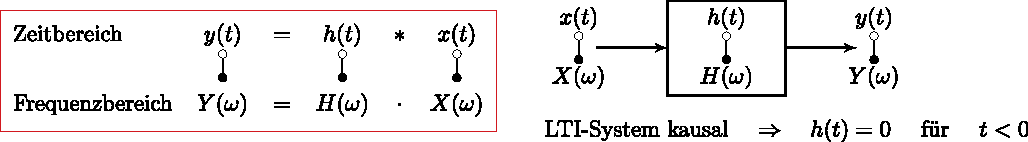
\includegraphics{chapters/05_LTI/figures/Faltung_System.pdf}

\subsection{Übertragungsfunktion \texorpdfstring{$H(\omega)$}{H(ω)}}

Fourier-Transformierte der Impulsantwort $h(t)$; beschreibt, wie das LTI-System jede Frequenz verstärkt und phasenverschiebt:
\efbox[linecolor=red]{$H(\omega) = \mathcal{F}\{h(t)\} = \frac{Y(\omega)}{X(\omega)} = |H(\omega)| \cdot e^{j\varphi(\omega)}$}
\quad mit \; $y(t) = x(t) * h(t) \;\laplace\; Y(\omega) = X(\omega) \cdot H(\omega)$.

\begin{tabular}{ll}
	$|H(\omega)|$: Amplitudengang & $\varphi(\omega) = \arg \left(H(\omega)\right)$: Phasengang.\\[1em]
	$|H(\omega)| \, [\text{dB}] = 20 \cdot \log{|H(\omega)|}$ & 
	$|Y(\omega)| \, [\text{dB}_R] = |H(\omega)| \, [\text{dB}_R] + |H(\omega)| \, [\text{dB}]$
\end{tabular}


\subsection{Verzerrungsfreies LTI-System S.39}
Ein LTI-System ist verzerrungsfrei, wenn das Ausgangssignal nur skaliert und verzögert ist: $y(t) = k_a \cdot x(t - t_d)$. Mit dem Verschiebungssatz folgt \efbox[linecolor=red]{$H(\omega) = k_a \cdot e^{-j\omega t_d}$}.
\begin{itemize}
	\item \textbf{Amplitudengang konstant:} $|H(\omega)| = k_a$, damit alle Frequenzanteile gleich stark verstärkt werden.
	\item \textbf{Phasengang linear:} $\varphi(\omega) = -t_d \cdot \omega$, damit alle Frequenzanteile um dieselbe Zeit $t_d = -\frac{\varphi(\omega)}{\omega}$ verzögert werden. Gleichwertig: die Gruppenlaufzeit $\tau_g = -\frac{d\varphi}{d\omega} = t_d$ ist konstant.
	\item \textbf{Kausalität:} $t_d > 0$, der Phasengang fällt daher linear mit steigender Frequenz ab.
\end{itemize}
In der Praxis genügt es, wenn beide Bedingungen innerhalb der Bandbreite des Signals erfüllt sind.

\subsection{Dirac Impuls (Stösschen) S.13}
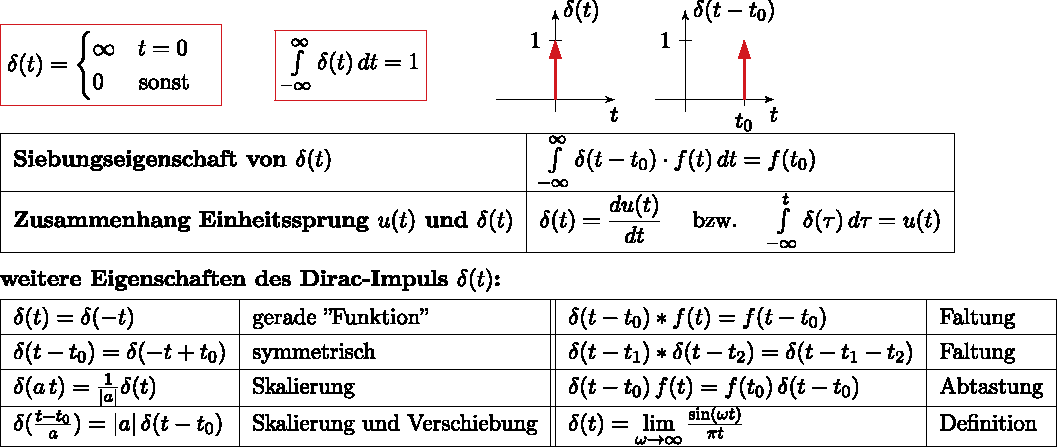
\includegraphics[width=.95\linewidth]{chapters/05_LTI/figures/stoesschen.pdf}

\subsection{Signalmanipulationen}
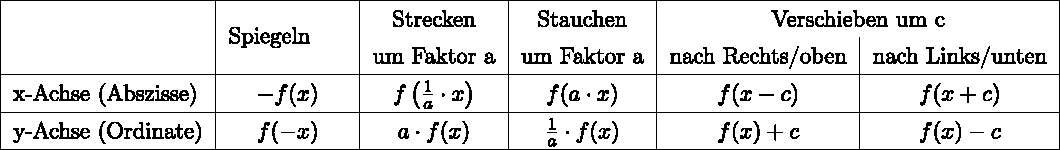
\includegraphics[width=\textwidth]{chapters/05_LTI/figures/signalmanipulation.pdf}

\subsection{Grundlegende Funktionen S.13}
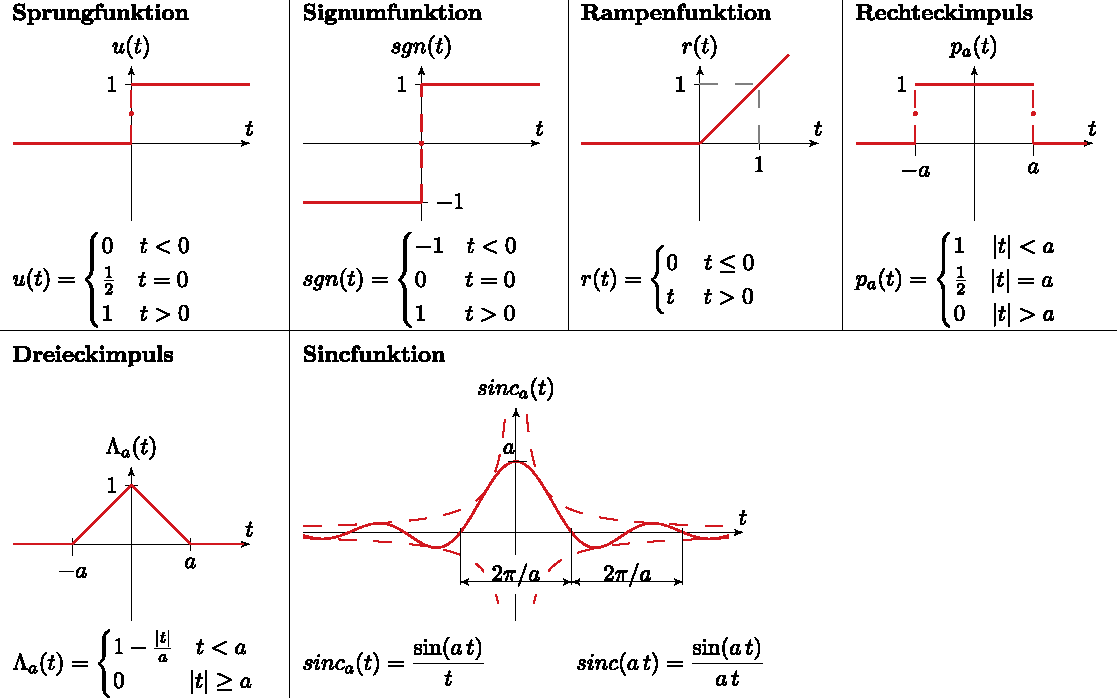
\includegraphics[width=\textwidth]{chapters/05_LTI/figures/grundlegende_funktionen.pdf}

\subsection{Filtereigenschaften von LTI Systemen S.39}

\begin{minipage}{.28\linewidth}
	\begin{center}
		\begin{tabular}{|c|c|c|}
			\hline
			Tiefpass & Lowpass & LPF \\
			\hline
			Hochpass & Highpass & HPF \\
			\hline
			Bandpass & Bandpass & BPF \\
			\hline
			Bandsperre & Bandstop & BSF \\
			\hline
		\end{tabular}
	\end{center}
\end{minipage}
\begin{minipage}{.71\linewidth}
	Ideale Filter sind \textbf{akausal} und deshalb \textbf{nicht realisierbar}. Reale Filter stellen einen Kompromiss dar:
	\begin{list}{$\bullet$}{\setlength{\itemsep}{0cm} \setlength{\parsep}{0cm} \setlength{\topsep}{0cm}} 
		\item Filterflankensteilheit (fianchi ripidi)
		\item Dämpfung im Sperrbereich (buona attenuazione in banda bloccata)
		\item Flachem Frequenzgang im Durchlassbereich (poca ondulazione in banda passante)
		\item Linearität des Phasengangs (fase lineare)
	\end{list}
\end{minipage}\vspace{-1em}

\subsubsection{Bandbreite}
Die Bandbreite ist nur für \textbf{Tiefpass und Bandpassfilter} definiert. Bei realen Filtern wird üblicherweise die \textbf{\qty{3}{\dB} Eckfrequenz} angenommen, dabei erreicht die Amplitudendämpfung einen Wert von $k=\frac{1}{\sqrt{2}}$

\begin{minipage}{.74\columnwidth}
	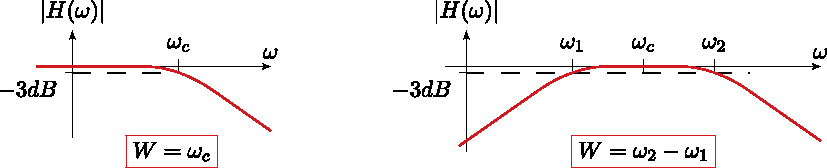
\includegraphics{chapters/05_LTI/figures/tiefbandpassbandbreite.pdf}
\end{minipage}
\begin{minipage}{0.25\columnwidth}
	\[\lvert H(\omega_c) \rvert = \frac{\sqrt{2}}{2} \cdot \lvert H(0) \rvert\]
	\[\lvert H(\omega_c) \rvert_{\rm dB} = \lvert H(0) \rvert_{\rm dB} - 3 dB\]
	Risolvere per $\omega_c$\medskip
	
\end{minipage}
\[|H|_{dB} = 20 \cdot \log\left(\frac{\omega}{\omega_c}\right) \qquad \text{Forme standard:} \quad
H_{\mathrm{LPF}}(\omega)=\frac{H_0}{1+j\,\omega/\omega_c},\quad
H_{\mathrm{HPF}}(\omega)=H_\infty\,\frac{j\,\omega/\omega_c}{1+j\,\omega/\omega_c}
\]

\subsection{Quadraturfilter, Hilberttransformation S. 43}
Der Quadraturfilter ist ein Allpassfilter, dieser lässt die Amplitude unverändert und dreht nur die Phase um eine viertel Periode $-\frac{\pi}{2}$. Es resultiert eine grosse Verzögerung für tieffrequente Anteile und eine kleine für hochfrequente Anteile.

\vspace{.03cm}
\begin{minipage}{.5\linewidth}
\efbox[linecolor=red]{$H(\omega) = -j \cdot sgn(\omega) = \left\{
	\begin{matrix}
		e^{-j\pi /2} \;\; \omega > 0\\
		e^{+j\pi /2} \;\; \omega < 0
	\end{matrix}
	\right.$}
\end{minipage}
\begin{minipage}{.5\linewidth}
	\vspace{.03cm}
	\hspace{.01cm}
	\efbox[linecolor=red]{$h(t) = \frac{1}{\pi \cdot t}$}
\end{minipage}\medbreak

\[{x}(t) = x(t) * \frac{1}{\pi t} = \frac{1}{\pi} \int_{-\infty}^{+\infty} \frac{x(\tau)}{t-\tau}\, d\tau 
\qquad 
{X}(\omega) = X(\omega) \cdot H(\omega) = -j \cdot \operatorname{sgn}(\omega) \cdot X(\omega)\]